\documentclass[aspectratio=169]{beamer}
\usetheme{Madrid}
\usepackage[utf8]{inputenc}
\usepackage[T1]{fontenc}
\usepackage{tikz}
\usepackage{amssymb}
\usepackage{graphicx}
\setbeamertemplate{navigation symbols}{}
\setbeamercolor{title}{fg=white,bg=magenta!70!red}
\setbeamercolor{frametitle}{fg=white,bg=magenta!70!red}
\setbeamercolor{block title}{bg=magenta!70!red!20,fg=black}
\setbeamercolor{block body}{bg=magenta!70!red!8,fg=black}
\setbeamercolor{item}{fg=magenta!70!red}
\setbeamercolor{itemize item}{fg=magenta!70!red}
\setbeamertemplate{itemize item}[triangle]

\title{Foundations 4 — Binary in Code \& Logic}
\subtitle{Real binary conversion, Boolean logic (AND/OR/NOT), and data types}
\author{ByteForge --- Grade 9 --- The Deep Diver}
\date{}

\begin{document}

\begin{frame}
    \titlepage
\end{frame}

\begin{frame}{Today's Missions}
    \Large
    \begin{itemize}
        \item Denary to Binary
        \item Binary to Denary
        \item Learn: Boolean Logic
        \item AND Gate
        \item Truth Table Row
        \item Learn: Data Types
        \item Pick the Type
        \item Type Coercion Trap
    \end{itemize}
\end{frame}

\begin{frame}{Converting a number INTO binary, in real code}
    \large
    \begin{itemize}
        \item Same powers-of-2 idea as the unplugged cards, now done with \texttt{bin(n)} in real code
        \item 22 becomes the text \texttt{"10110"} --- notice it comes back as a STRING, not a number
    \end{itemize}
\end{frame}


\begin{frame}{AND, OR, NOT --- the three basic logic operators}
    \large
    \begin{itemize}
        \item AND --- true only if BOTH sides are true (the strictest one)
        \item OR --- true if AT LEAST ONE side is true (the most generous one)
        \item NOT --- simply flips a value: True becomes False, and back again
    \end{itemize}
\end{frame}


\begin{frame}{A truth table checks every possible combination}
    \large
    \begin{itemize}
        \item Work compound expressions like brackets in maths: innermost first
        \item \texttt{NOT (a AND b) OR c} --- do the AND, then NOT it, THEN the OR
    \end{itemize}
\end{frame}


\begin{frame}{Every value has a real, specific data type}
    \large
    \begin{itemize}
        \item integer (whole number), real/float (decimal), string (text), boolean (True/False)
        \item \texttt{"7"} and \texttt{7} are genuinely different types even though they look almost identical
        \item Coercion = converting a value from one type to another ON PURPOSE, e.g. \texttt{int("42") + 8}
    \end{itemize}
\end{frame}

\begin{frame}{Real-World Examples}
    \large
    \begin{itemize}
        \item A car will only start (AND logic) if the key is turned AND the door is shut AND it is in park --- every condition genuinely has to be true.
        \item A house alarm triggers on OR logic --- ANY door OR ANY window opening sets it off, not all of them at once.
    \end{itemize}
\end{frame}


\begin{frame}{Image}
    \begin{center}
    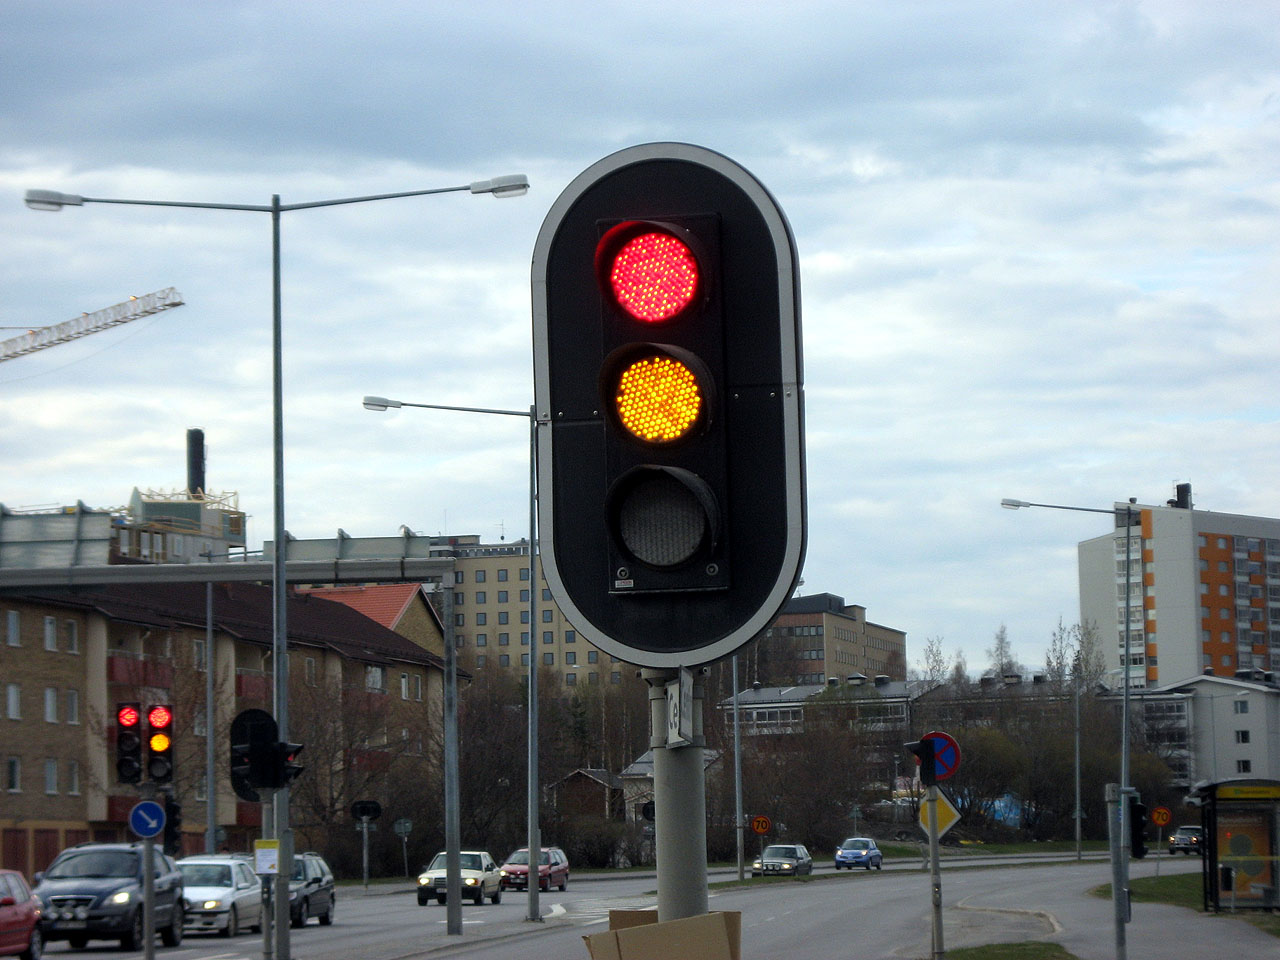
\includegraphics[width=0.5\textwidth]{images/traffic.jpg}

    \large A real traffic light is a genuine 3-way logic decision, running on rules exactly like AND/OR/NOT.

    \small LED traffic lights, public domain (PD-self), via Wikimedia Commons
    \end{center}
\end{frame}

\begin{frame}{Let Them Discover (1/2)}
    \large
    Think of a real rule at home or school that uses AND ("you can go out if homework is done AND it is before 6pm"). Which parts have to BOTH be true?
\end{frame}


\begin{frame}{Let Them Discover (2/2)}
    \large
    Find a real rule that uses OR instead ("bring an umbrella if it is raining OR very cloudy"). How is that different from an AND rule?
\end{frame}

\begin{frame}{Your Turn}
    \Large
    Open the mission map, find \textbf{Foundations 4 — Binary in Code \& Logic}, and fly it for real ---
    everything you just saw, you now do yourself.
\end{frame}

\end{document}
